% git-ui-thesis.tex
% Created: 3/4 2015

%\documentclass[12pt,a4paper,article,compsoc]{IEEEtran}
%\hyphenation{op-tical net-works semi-conduc-tor}
\documentclass[a4paper,oneside]{bth} % I WANT "twocolumn"!!!
\usepackage{paralist}
\usepackage{cite}
\usepackage{hyperref}
\usepackage{float}
\usepackage{tabu, tabularx, caption, subcaption}
%\usepackage{graphicx}

\usepackage{amsmath}
\usepackage{mathenv}
\usepackage{amssymb}
\usepackage{amsthm}
\usepackage{textcomp}
\usepackage{longtable}
\usepackage{multirow}
\usepackage{pifont}
\usepackage{changepage}
\usepackage{listings}
\usepackage{url}
\usepackage{xspace}
\usepackage{xtab}
\usepackage[utf8]{inputenc}
\usepackage[T1]{fontenc}
\usepackage{graphicx}
\DeclareGraphicsExtensions{.pdf}

\begin{document}
		\pagestyle{plain}
		\pagenumbering{roman}
		
		% Front matter
		{\pagestyle{empty}
		\changepage{5cm}{1cm}{-0.5cm}{-0.5cm}{}{-2cm}{}{}{}
		\noindent%   
			{\small
				\begin{tabular}{p{0.75\textwidth} p{0.25\textwidth}}
					\textit{Bachelor Thesis}&\multirow{4}{*}{\bthcsnotextlogo{3cm}}
					\\
					\textit{Computer Science}
					\\
					%\textit{Thesis no: MCS-2015-NN}
					\\
					\textit{06 2015}
					\\
				\end{tabular}
			}
			\begin{center}
				\par\vspace {7cm}
				{\Huge\textbf{Working with git user-interfaces}}   
				\par\vspace {0.5cm}
				{\Large\textbf{Centered Subtitle Times Font Size 16 Bold}}                   
				\par\vspace {3cm}
				{\Large\textbf{Robin Olofsson}}
				\\
				{\Large\textbf{Sebastian Hultstrand}}
				\par\vspace {7cm}
			\end{center}

			\noindent%
			{\small Dept. Computer Science \& Engineering 
			\\
			Blekinge Institute of Technology
			\\
			SE--371 79 Karlskrona, Sweden}
			\clearpage
		}

		{\pagestyle{empty}
			\changepage{5cm}{1cm}{-0.5cm}{-0.5cm}{}{-2cm}{}{}{}
			\noindent%
			\begin{tabular}{p{\textwidth}}
				{\small This thesis is submitted to the Department of Computer Science \& Engineering at Blekinge Institute of Technology in partial fulfilment of the requirements for the degree of Master of Science in Computer Science. The thesis is equivalent to 20 weeks of full-time studies.}
			\end{tabular}
			\par\vspace {12cm}
			\noindent%
			\begin{tabular}{p{0.5\textwidth}lcl}
				\textbf{Contact Information:}\\
				Author(s):
				\\
				Robin Olofsson
				\\
				E-mail: \url{Olofsson_@live.se}
				\\
				Sebastian Hultstrand
				\\
				E-mail: Sebastian@storm-net.se
				\\
				\par\vspace {5cm}
				University advisor:
				\\
				Prof.\ Conny Johansson
				\\
				Dept. Computer Science \& Engineering
				\par\vspace {1cm}
				\noindent%
 				\\
				Dept. Computer Science \& Engineering & Internet & : & www.bth.se/didd\\
				Blekinge Institute of Technology & Phone	& : & +46 455 38 50 00 \\
				SE--371 79 Karlskrona, Sweden & Fax & : & +46 455 38 50 57 \\
			\end{tabular}
			\clearpage
		} % Back to \pagestyle{plain}

		\setcounter{page}{1}

		% ABSTRACT
		\abstract
		\begin{changemargin}{+1cm}{+1cm}
			\noindent
				Abstract goes here.

			\par\vspace {1cm}
			% 3-4 keywords, maximum 2 of these from the title, starts 1 line below the
			% abstract.
			\noindent
			\textbf{Keywords:} 3-4 keywords, maximum 2 of these from the title, starts 1 line below the abstract.
		\end{changemargin}

		\tableofcontents 
		\listoffigures %in case you have them
		%\listoftables %in case you have them
		%\listofalgorithms %in case you have them

		\cleardoublepage
		\pagestyle{headings}
		\pagenumbering{arabic}
		
		% Settings of author and title
		\title{This title is not determined yet}
		\author{Robin~Olofsson and Sebastian~Hultstrand}
		
		% Content
		\chapter{Introduction}
		Git is a very popular version control system out there today along with systems like SVN and Mercurial. And the discussions between using CLIs' (Command-line interfaces) or GUIs' (Graphical user interfaces) in general have been going on since the late 70's and early 80's when operating systems like the Lisa and Macintosh among others came out \cite{HistoryOfGUIWiki} and the GUI revolution was kicked into high gear.
		To date people seem to prefer the CLI over GUI when working with Git, however it is not clear as to why.
		Theories do exist which state that the CLI provides a faster and more controlled way of dealing with Git. \cite{GitUserSurvey}\cite{GitInClassroom}
		\\
		The reason this topic was thought of in the first place is due to an observation made in one of our classes. As of the day of writing there is no real formal introduction course to version control at Blekinge Institute of Technology, much less to Git. So instead there are a small number of courses where students are introduced to git alongside the actual content of the course and most of the learning is left to what the student chooses to find out.
		During one of these introduction talks about git the students were encouraged to start out by using the command-line interface in order to get a feel for how git works. This was met by a lot of complaining from the students as they would rather use one of the graphical user interfaces. The subsequent discussion that ensued was the spark that lit the idea to do this research.
		\\
		In this paper a closer look is taken into what people use today, in terms of interfaces to work with Git, and if there's any correlation to be found between how people use Git and which interface is used to do so.
		The aim is to find out which interface is more preferred, which is more suitable to novice users and if developers can benefit more from using either of the two interfaces when reaching a certain knowledge-level of Git.
		To find these answers we have conducted a survey, through an online service, that has been sent out to developers within the industry and students at Blekinge Institute of Technology.
		A literature study has been carried out as well, mainly to help  gather as much knowledge about current opinions within the scientific scene about the CLI and GUI interfaces.
		The results of the literature study enabled the creation of a  survey and after further development of the questions, used in the survey, a small number of interviews were conducted to get a deeper understanding of the choices made.
		We felt that a survey might provide enough information to carry out the work but by conducting interviews too a better understanding could actually be reached as to why the participants of the survey answered the way that they did.
		
		% Background
		\chapter{Background}
			\section{Git}
			In 2005 the Linux development community started the development of Git.
			Up until that point they had been using BitKeeper as their version control system. By that time BitKeeper was free but when the company behind the product decided to price it the Linux development community quickly abandoned the solution to develop their own open-source version control system.\cite{ProGit}
			To date, Github alone has over 21.7 million repositories.\cite{GithubAbout} All of these repositories are, as might be obvious, Git repositories. 
			Git is, today, one of the most common version control systems \cite{EclipseDeveoperReport}\cite{DeveloperProductivity}\cite{MicrosoftSurveyResults}. The reason for git being a vary powerful tool is its flexibility, the core is well designed and quite ingenious and the surrounding functionality is adaptive and highly customizable. This contributes to two things, the learning curve being quite steep and a challenge to get over and second once you get over the curve you can very easily navigate the functionality and structure of a git repository and have little difficulty learning new methods and work flows. This at least seems to be the consensus on forums and message boards around the web, and it coincides quite accurately with our experiences as well.
			\\
			The basic structure of a git repository is; 1) a .git directory that houses the meta date and object database for your repository and all the committed changes. 2) A staging area where changes that are to be committed are kept in waiting for a commit to take place. 3) A working directory where your plain working copy of the source code is held. This is where development is done. \cite{GitStructure} 
			So depending on what version of the code you checkout from the .git directory, it will appear in the working directory. Then you code your changes and stage them, thus placing the changes securely in the staging area. Then the final step is to commit what is in the staging are and it will get saved into the .git directory. Then some repositories also have a remote host that the changes can be pushed to for ease of sharing the code. Those are the very basics of how git works \cite{GitStructure}
			
			\section{Command-line interface and the Graphical user interface}
			There are two main ways of interfacing with Git, one is through a command-line interface and the other is through one of many graphical user interfaces. \cite{GitGUIs}\\
			
			When using the command-line interface you type commands manually to preform the desired actions whilst in the graphical user interface you will have something visual to interact with, such as buttons, input fields and so on.
			There's pros and cons with using either of the two interfaces not only for git but in general.
			For example, through a command-line you can perform some actions, like renaming 100 files with a lot less effort than with a graphical user interface but it would require you to know the commands needed to rename the files. One command can perform a lot of different tasks, whilst in a graphical user interface you would normally have to rename each file one by one which would require a lot more time but less knowledge. As mentioned in the introduction the debate of GUI v. CLI has been going on since the 80's and not a great deal has changed in the arguments, since they are so deeply ingrained in either interface. 
			A good analogy is the car dealership comparison made in the article (Later a book) \textit{In the beginning was the command-line} (Stephens, 1999) \cite{InTheBeginning}. The summary of the analogy would be that there are a bunch of competing automotive dealerships on the same street where some are expensive, but easy to use and fairly cheep to repair however they often break down. Another sells sleek euro-style cars that no one really knows the inner workings of, they are expensive but beautiful. Then there is the super advanced tanks that are being given away for free. Yet still all the customers go for the cheap car that is sort of bad or the expensive euro-car. No one wants a tank even though they are free, because no one can be bothered to learn how to drive it. 
			This analogy helps to illustrate the situation between the GUI and CLI very simply but quite accurately. 
			
			\section{Technical terms}
			Below there is an explanation to common terms that will be used throughout this paper.
			
			\subsection{CLI}
			CLI means command-line interface, which is a way to interact with a computer and perform certain tasks by typing commands into a text based interface, as depicted in figure 2.1.
			\begin{figure}[p]
				\centering
				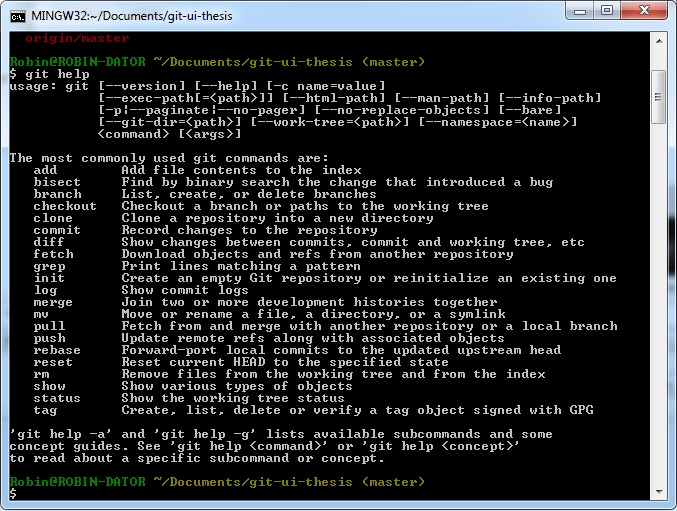
\includegraphics[width=0.8\linewidth]{git-cli.jpg}
				\caption{Git command-line interface, in Windows}
				\label{fig:git-cli}
			\end{figure}
			
			\subsection{GUI}
			GUI means graphical user interface. A graphical user interface is a program interface that takes advantage of the computer's graphics capabilities to make a the program easier to use \cite{WhatIsGui}, by way of human relatable representations and structures. An example of such an interface for git can be seen in figure 2.2.
			\begin{figure}[p]
				\centering
				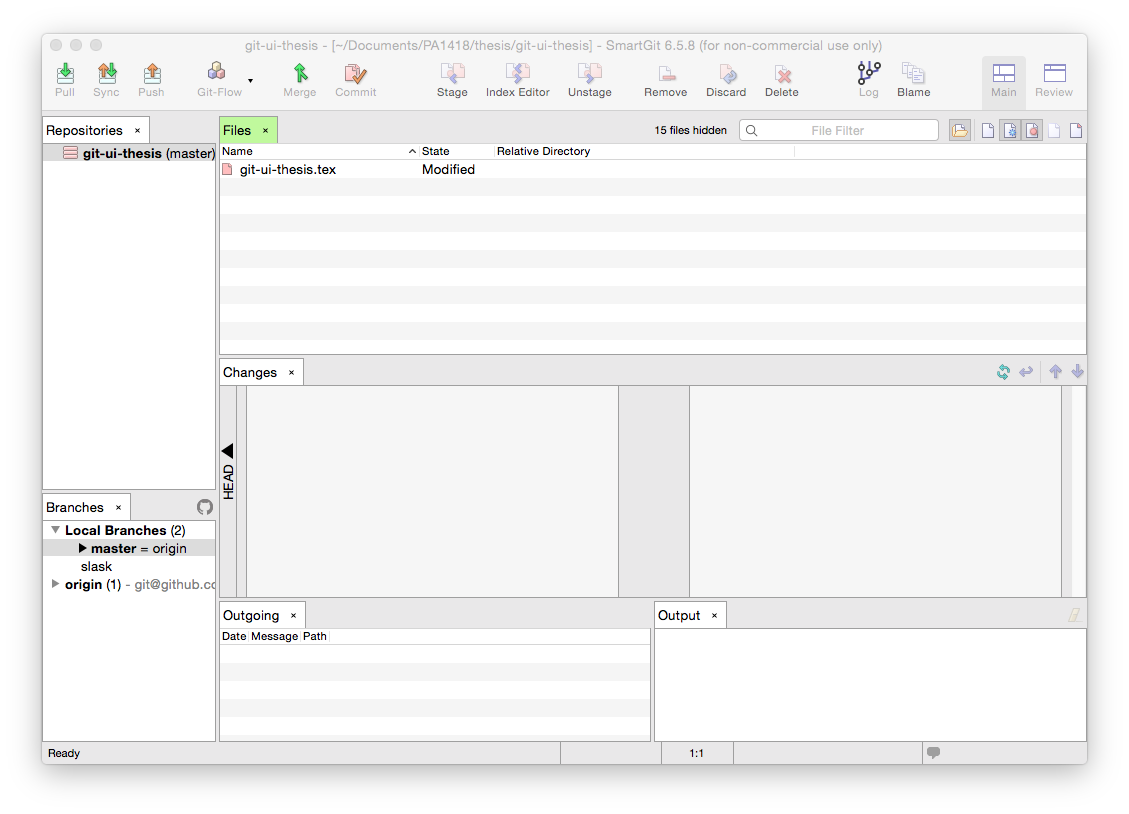
\includegraphics[width=0.8\linewidth]{git-gui.png}
				\caption{Git graphical user interface, Smart Git Hg on OSX}
				\label{fig:git-gui}
			\end{figure}
			
			\subsection{VCS (Version Control System)}
			A VCS usually consists of two applications, one on a server-side and one on a client-side.
			It's basic functionality is to maintain source code, other types of software files and their history.\cite{FoundationVCforWebDevs}
			
			\section{Terminology used}
				\begin{itemize}
					\item Demographic - The word demographic is used in this thesis and refers to a certain group that answered our survey. The groups members are defined by their indicated level of proficiency with git, and the amount of time they have worked with git. The determination of which demographic a respondent falls in is made up of a point system. The alternatives are given an arbitrary point value to signify rank and when the points for the chosen alternatives are added up we get the sum for the respondent. Low is defined as 2-4, mid 5-7 and high 8-9. We did this in order to make it possible to split the respondents into demographics.
					\item UI - The word is an abbreviation of the term user interface and refers to either the graphical user interface, command-line interface or both.
				\end{itemize}
			
		% Research methodology
		\chapter{Research methodology}
			\section{Research questions}
			\begin{enumerate}
				\item What is most commonly used when getting started with git, CLI or GUI?
				\item What is most commonly used by experienced git users, CLI or GUI?
				\item What can be gained from using the GUI, in the aspects of functionality and convenience?
				\item What can be gained from using the CLI, in the aspects of functionality and convenience?
				\item At what stage of git proficiency would you stand to gain the most from the CLI or the GUI? (Looking at what should you start out with to learn how git works and how it is used, and what you will gain the most from when you get to a higher level of understanding git.)
			\end{enumerate}
		
			\section{Approach for answering research questions}
			To answer the research questions a literature study was conducted to find out how git works, Git work-flows and discussions about the command line interface and the graphical user interface in general. Based on what is found, a design of a survey and a number of  questions for interviews was created.\\
			The intention of the survey is to collect information about current users preferences and perceptions. We want to know what they are currently using (either CLI or GUI tool), how long they have been using it, what their perception of the two different types of interface is, how they work with git, how they began using it and how they learned to use it. This to find correlations between their experience with and use of git, to their preferences and reasoning behind their choice of tool.\\
			The interviews will be based on more open questions where the aim is to allow the subject to elaborate around why they have chosen to work like they do, and discuss the perks of the two different types of interfaces that we put forward. The aim of the exercise is to get a deeper understanding of the reasoning that goes into the choice, an understanding that the survey will not be able to supply.\\
			Thirdly we will also be looking at examples of the UIs to make an assessment of what users can gain from the particular interface in tearms of functionality and convenience. We will look at the CLI tool in a Linux environment, the GUI based tools Sourcetree and Smart Git Hg, both of which are available for the three large platforms (Windows, Mac and Linux).\\
			Studies have been conducted to try to find out what people use when interfacing with Git, but the most recent study to cover that area, that we could find was conducted in 2012.
			By conducting a survey, where we aimed to find out what people use today and why, there was the possibility to gather fresh data as the data collected back in 2012 might not accurately represent how people interface with git today.
			\\\\
			In summary questions 1 and 2 will be answered in the survey where questions pertaining to what UI the subject is currently using and what UI the subject started using Git in. Correlations will also be searched for in the 2012 GitSurvey \cite{GitUserSurvey} to see how the results compare to other studies.
			Questions 3 and 4 will be answered in part through some of the perception related questions in the survey coupled with the interviews and most of all the analysis conducted on the UIs mentioned above. Finally question 5 will be answered by, in part, statistics from the survey by looking at questions pertaining to perception of the UIs, time consumption associated with the subjects use of git, both general and problem based, and the subjects varying use of and proficiency with git. Also partly through the interviews where being able to hear what drew the subjects to the UI that they use, what they believe to be important in the choice and their thoughts about what was found during the UI analysis. Since we will be able to determine demographics based on the level of proficiency, from the survey. We can use those to find and interview subjects that can represent a certain demographic and discuss their needs and requirements from the user interfaces. Looking at the results from that coupled with the findings from the analysis of Linux CLI tool for git, SourceTree and Smart Git Hg will lead to a comprehensive answer to the 5th research question that takes the demographics needs and preferences into account.  
			Our belief is that, by answering questions 1 to 5, developers will get a general overview of how todays Git users interface with Git and why. The "why" doesn't have to be detailed for the information to be valuable because it might be enough to know that, hypothetically, making a commit and pushing code through the graphical user interface is slower than doing the same in the command-line interface.  
		 
			\section{Literature review design}
			In our literature study we used the following search engines:
			\begin{itemize}
			\item BTH Summon
			\item Engineering Village
			\item IEEE Xplore
			\item Google scholar
			\end{itemize}
			The keywords we used was:
			\begin{itemize}
			\item git
			\item configuration control
			\item version control
			\item public domain software
			\item software engineering
			\item linux
			\item UI
			\item User interface
			\item Graphical user interface
			\item GUI
			\item CLI
			\item Command line interface
			\item Case study
			\item User experience
			\item Usability
			\item UX
			\item Interface
			\end{itemize}
			
			To sort out what literature that was relevant we had to read the abstracts.
			Whenever we found a literature that had a relevant abstract we would then proceed to add it to a stack with literature that we believed to be relevant to our work.
			After getting roughly 10 papers we started snowballing in hope of finding more relevant papers.
			
			\section{Empirical study design}
			
				\subsection{Survey}
					\subsubsection*{Goal with the survey}
					The survey consists of 13 multiple choice questions, the questions are aimed to be as easy and quick to answer as possible in order to persuade people to answer the survey. What the survey is aimed at finding out is the following; the level of experience the subject has with git, what UI they are currently using, what they have used in the past and if there is a specific reason for why they use the interface that they use. We also want to find out how the subject learned to use git, what they primarily use Git for, what operating system they are working on and how much time they spend on average interacting with Git as part of their development work. Finally we want to get some insight as to how often they need to consult another person or resources online or in handbooks to solve issues that arise in Git, accompanied with some word association with the two different UI types to get a statistical view of how the users perceive them.
					
					\subsubsection*{Questions and alternatives}
					\begin{enumerate}
						\item How long have you been working with git?\\
						\begin{inparaenum}[\itshape a\upshape)]
							\item \textless 6 months
							\item 6 months - 1 year
							\item 1-3 years
							\item 3-5 years
							\item 5-10 years
						\end{inparaenum}
						\item How would you rate your knowledge of git?\\
						\begin{inparaenum}[\itshape a\upshape)]
							\item Novice
							\item Average
							\item Professional
							\item Master
						\end{inparaenum}
						\item What type of user interface are you primarily using for git?\\
						\begin{inparaenum}[\itshape a\upshape)]
							\item Command-line interface
							\item Graphical user interface
							\item Both equally
						\end{inparaenum}
						\item How did you learn to use git?\\
						\begin{inparaenum}[\itshape a\upshape)]
							\item Colleague or friend
							\item Open source community
							\item Online tutorials
							\item Book
							\item Course
							\item Self taught
						\end{inparaenum}
						\item What interface did you use when starting out with git?\\
						\begin{inparaenum}[\itshape a\upshape)]
							\item Command-line interface
							\item Graphical user interface
						\end{inparaenum}
						\item Why do you use the interface you use today?\\
						\begin{inparaenum}[\itshape a\upshape)]
							\item Personal preference
							\item Standards for work environment
							\item Outside influences
							\item It is what i know best
						\end{inparaenum}
						\item What operating system do you primarily use?\\
						\begin{inparaenum}[\itshape a\upshape)]
							\item Windows
							\item Mac
							\item Linux
						\end{inparaenum}
						\item What do you mainly use git for?\\
						\begin{inparaenum}[\itshape a\upshape)]
							\item Basic change tracking
							\item Collaborative work
							\item Large scale version control with branch management and code reviewing through git
						\end{inparaenum}
						\item How many minutes per hour of development time, on average, do you spend on interfacing with git?\\
						\begin{inparaenum}[\itshape a\upshape)]
							\item \textless 5 min
							\item 5-10 min
							\item 10-15 min
							\item 15-20 min
							\item 20-25 min
							\item 25-30 min
							\item \textgreater 30 min
						\end{inparaenum}
						\item How many times during a work day do you need to seek help for an issue with git?\\
						\begin{inparaenum}[\itshape a\upshape)]
							\item 0
							\item 1-2
							\item 2-4
							\item 4-6
							\item 6-10
							\item 10-15
							\item 15-20
							\item \textgreater 20
						\end{inparaenum}
						\item What words do you associate with a Git GUI (Graphical user interface)?\\
						\begin{inparaenum}[\itshape a\upshape)]
							\item Aesthetic
							\item Easy
							\item Bulgy
							\item Auto-magic
							\item Difficult
							\item Helpful
							\item Simple
							\item Intuitive
							\item Insightful
							\item Hard
							\item Time consuming
							\item Cool
							\item Professional looking
							\item Control
							\item Difficult
							\item Ugly
							\item Old fashioned
						\end{inparaenum}
						\item What words do you associate with the Git CLI (Command-line interface)?\\
						\begin{inparaenum}[\itshape a\upshape)]
							\item Aesthetic
							\item Easy
							\item Bulgy
							\item Auto-magic
							\item Difficult
							\item Helpful
							\item Simple
							\item Intuitive
							\item Insightful
							\item Hard
							\item Time consuming
							\item Cool
							\item Professional looking
							\item Control
							\item Difficult
							\item Ugly
							\item Old fashioned
						\end{inparaenum}
						\item Which type of Git interface would you recommend others to use, no matter skill level?\\
						\begin{inparaenum}[\itshape a\upshape)]
							\item Command-line interface
							\item Graphical user interface
							\item Both
						\end{inparaenum}
					\end{enumerate}
				
					\subsubsection*{Crafting and distribution}
					The survey will be made as a web form that we can easily collect the data from and most of all distribute easily. Distribution of the survey is done through a number of different channels online such as BTH:s student mail list, through contacts at different Swedish companies, trough large companies that work with git that we have been able to procure assistance with and finally 3-7 [EXACT NUMBER LATER] different sub-reddits (Forum boards at the popular web forum Reddit) associated with software development.
					To get as many responses as possible the survey is designed to be easy and quick to fill out and there is also going to be a lottery draw among the participants for three, one month gift subscriptions to the curio service Loot Crate. \cite{lootcrate} 
				
					\subsubsection*{Analysis of survey}
					The survey is crafted so that it can be evaluated and analysed in conjunction with the interviews. 
					First a demographic for the replying party will be determined based on their answers to questions one and two. This demographic will be used when looking at the questions about what user interface they use and have used, their reasoning for using it and their perceptions of the user interfaces. The demographic is necessary to determine since the fifth research question is based on both experienced and inexperienced users. The interviews are designed in a way that will give more insight into the reasoning and perceptions of a certain demographic, but this is explained further in the Interviews chapter.
					\\
					Questions three and five will be directly used to determine the answer to the first research question and in conjunction with the determined demographic to answer the second research question.
					\\
					The rest of the questions on the survey (Questions 4, 6 - 13) are used as factors for answering the third, fourth and fifth research questions. As they pertain to difficulties, perceptions and opinions about the user interfaces. When coupled with the results from the interviews and the study of the user interfaces mentioned in section 3.2, they will place weight on elements that are found, thus allowing the determination of what parts of a user interface to git, that the different demographics value or are influenced by. Graphs will be crafted in order to easily convey the messages that the collected data holds. For example bubble graphs to look at how the different demographics are responding to the word association questions to find relationships between ability and perception of the interface type. 
					\\
					The data that was collected through the survey was stored in a Google spreadsheet \cite{GoogleSpreadsheet} and through that spreadsheet we parsed the resulting XML (Exstensible Markup Language) into a MySQL database where querying the data to build datasets for graphs is a lot easier.
					Through the diagrams we could easily find out percentages of how many answered a question in a certain way and through that we could draw conclusions to help us in answering the research questions.
					
				
				\subsection{Interviews}
				The interviews are conducted with a small group of subjects that are representative of a certain demographic that answer the survey. The way that a demographic is determined in this context is the level of proficiency with git that the subject indicates and how long the subject has been using git for. 
				These two aspects will allow analysis on a deeper level, of the needs and wants of different users. The minimum demographics to cover are new users of git whom are learning to use git at the moment and experienced users whom have used git often and for a long time. The identifiers for these two groups are;
				\begin{itemize}
					\item[Group 1 - New users.]
					These users have less than one year of experience and identify them selves as Novice or Amateur users.
					\item[Group 2 - Experienced users.]
					These users have more than two years of experience and identify them selves as Pro or Master users.
				\end{itemize}
					\subsubsection*{Interview format}
					The format of the interviews will be a discussion on the topic of this paper where the aim is to get the subjects to explain their standing on the issue of CLI v. GUI in git interaction, and most of all elaborate around perceptions and experiences that they have. We will also supply some information about the UI:s to allow the sessions to go into as much detail as possible. 
					We will conduct 3 interviews with a students new to git and professionals using git every day, the sessions will be recorded and transcribed later to minimize the loss of information.
					
					\subsubsection*{Questions and topics to discuss}
						\begin{itemize}
							\item What functionalities do you most often use?
							\item How do you perceive working with a Git GUI?
							\item How do you perceive working with Git CLI?
							\item Which, if any functionality do you miss in the interface you use today? In terms of ease of use, efficiency and comfort.
						\end{itemize}
						
						These questions are aimed at finding out more about what the subject needs and wants from the interface he or she works with. However factors that need to be taken into account when looking at this are how much the subjects knows about the interfaces, what type of work they actually do in Git and if the work is collaborative or not. These factors are covered in either the responses to the survey or the interview it self and will be taken into account in the discussion.
				\subsection{User interface analysis}
				The analysis will not be conducted according to any usability metrics or heuristics scale. The analysis will consist of looking at what is possible to do in either of the interfaces, functionality and ability to customize behaviour in order to optimize the way you work with the interface. Since the interfaces are very different and we do not possess the knowledge and tools needed we will not take aesthetics into account. Since the graphical user interfaces and the command-line interface have a basic set of functionality that are going to perform roughly the same tasks we will not take the basic functions into account, like staging, committing, merging, pushing, pulling, cloning and so on.
				The analysis will be a simple high level overview of the haves and don't-haves of the interfaces, basically a pros and cons list, this in order to stay objective.
		
		% Literature study		
		\chapter{Literature review}
		
			\section{Command-line versus Graphical user interface}
			Based on what we found people with experience about Git will in most, if not all cases prefer the command-line interface over the graphical user interface.\\
			The reason behind this is however, not crystal clear.In the 2012 edition of GitSurvey \cite{GitUserSurvey}, about 97\% of the people who answered the question “What Git implementations do you use?”, use the git command-line whilst only 8\% use some graphical user interface.\\\\
			If we go back to a time, before git. A time when the concept of graphical user interfaces were quite new, there was a study conducted on students to see whether they would prefer the command-line interface over the graphical user interface. The study was done at Waikato University, New Zealand, back in 1992 and involved a mix of Macintoshes and IBM PC compatibles.\\
			A group of students were placed in front of these machines so that the staff was able to observe how they responded to interacting towards Macintoshes graphical interface and IBM PC compatibles command-line.\\
			The theory was that the students, whom had no prior computer experience, would prefer the Macintosh because of the fact that a graphical user interface has a less harsh learning curve than a command-line.This theory was also backed up by Morgan, et al \cite{MouseToRat} and Kirkpatrick et al \cite{MacVsWindows}.\\
			Based on this study and another, more git-focused study that was conducted in 2014 \cite{GitInClassroom}, the theory seems to be that graphical user interfaces would appeal to novice users more.\\
			However theoretically, as users get more and more experienced they will gradually start to prefer the command-line interface over a graphical user interface because they are able to complete their tasks faster and to maintain more control over what they are doing and what's going on.\\\\
			Now, lets forget about the theories and focus on what these studies yielded in the form of results. Generally speaking it would seem that a user tends to use what they find to be easier \cite{Treweek}. Because graphical user interfaces do have a more lenient learning curve it would therefore appear logical that a user would prefer that over a command-line interface. In terms of Git, graphical user interfaces are likely more valuable when the knowledge of the system matures for the user \cite{GitInClassroom}. Git is complex, if you check the answers for the question “What do you hate about Git?” in the 2012 edition of GitSurvey you will notice that this is one of the answers. Another answer to this question is ”requires steep learning curve for newbies”. This is what spurred the development of graphical user interfaces for Git, the goal was to hide some of Git:s complexity. \cite{WrongWithGit}
			
			According to Eric S. Raymond, the disadvantage of the commandline interface is that it almost always has high mnemonic load (low ease), and usually has low transparency. Most people (especially non-technical end users) find such interfaces relatively cryptic and difficult to learn. \cite{ArtOfUnixProgramming}
			Juergen Haas believes that the CLI is generally easier to use if you can remember the commands and options, which you probably would if you use them a lot. \cite{LinuxGuiVsCli}
			
			
			\section{Summary of the literature study results}
			The graphical user interfaces that are available for Git is a lot less used than the Git command-line. Yet people with low experience seem to prefer the graphical user interfaces because they appear to be easier to use. The people that answered the GitSurvey in 2012 was a group of mostly everyday users or more experienced than average users of Git \cite{GitUserSurvey}, so it is hard to judge whether the statement in the line above is valid or not but if you are to believe the previously introduced studies then it would make sense. After looking at the previous studies, we would have to say that command-line interfaces seem to be something that attracts more experienced users whilst graphical user interfaces attracts novice users.
		
		% Results	
		\chapter{Results}
			\section{Survey}
			The survey got 358 responses from people around the world whom use git in one way or another. The sizes of each demographic can be seen below in figure 5.1.
			\begin{figure}[H]
				\centering
				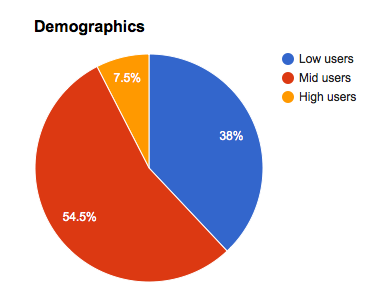
\includegraphics[width=0.5\linewidth]{graphs/demo_split.png}
				\caption{Graph showing the split among the demographics covered in the survey}
				\label{fig:graph-demo-split}
			\end{figure}
			Below follows graphical representations of how the respondents to the survey answered each question, these diagrams show the full spectrum of respondants as a whole. More in-depth graphs with different conditions will follow after that.
			\begin{figure}[H]
				\centering
				\begin{subfigure}[b]{0.45\textwidth}
					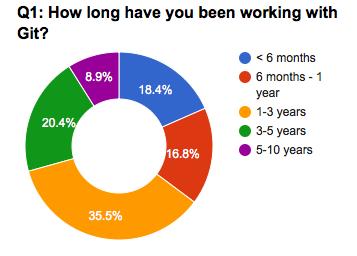
\includegraphics[width=\textwidth]{graphs/q1.png}
					\caption{Representation of results of question 1}
					\label{fig:q1}
				\end{subfigure}
				~
				\begin{subfigure}[b]{0.45\textwidth}
					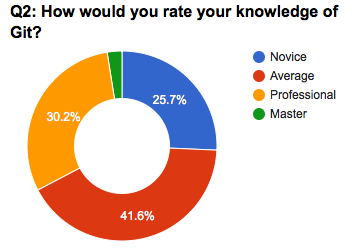
\includegraphics[width=\textwidth]{graphs/q2.png}
					\caption{Representation of results of question 2}
					\label{fig:q2}
				\end{subfigure}
				\caption{Questions 1 and 2}\label{fig:q1-q2}
			\end{figure}
			\begin{figure}[H]
				\centering
				\begin{subfigure}[b]{0.45\textwidth}
					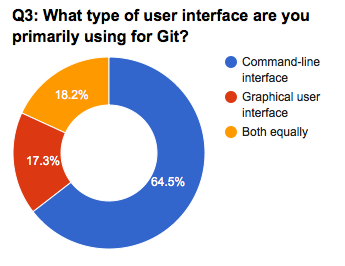
\includegraphics[width=\textwidth]{graphs/q3.png}
					\caption{Representation of results of question 3}
					\label{fig:q3}
				\end{subfigure}
				~
				\begin{subfigure}[b]{0.45\textwidth}
					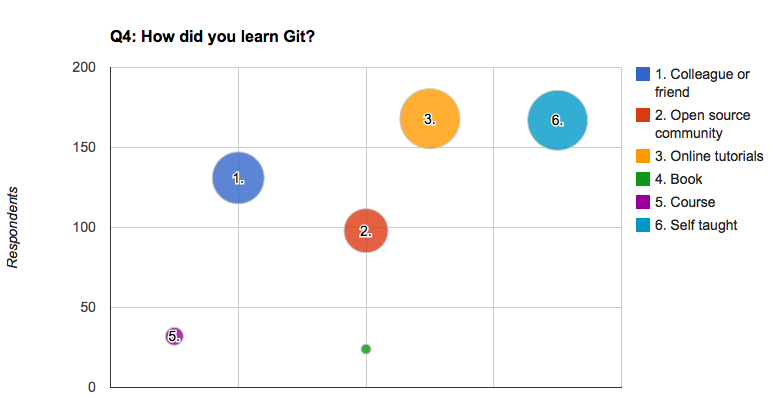
\includegraphics[width=\textwidth]{graphs/q4.png}
					\caption{Representation of results of question 4}
					\label{fig:q4}
				\end{subfigure}
				\caption{Questions 3 and 4}\label{fig:q3-q4}
			\end{figure}
			\begin{figure}[H]
				\centering
				\begin{subfigure}[b]{0.45\textwidth}
					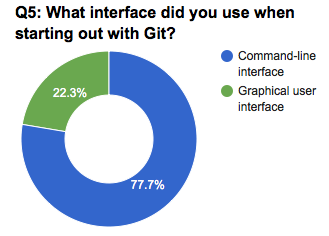
\includegraphics[width=\textwidth]{graphs/q5.png}
					\caption{Representation of results of question 5}
					\label{fig:q5}
				\end{subfigure}
				~
				\begin{subfigure}[b]{0.45\textwidth}
					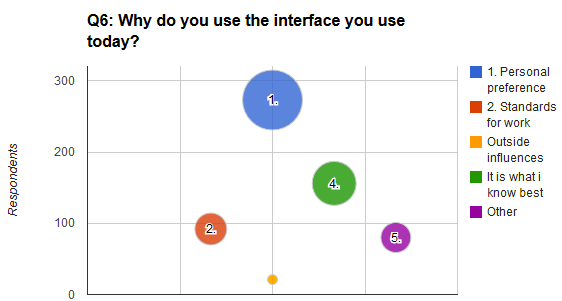
\includegraphics[width=\textwidth]{graphs/q6.png}
					\caption{Representation of results of question 6}
					\label{fig:q6}
				\end{subfigure}
				\caption{Questions 5 and 6}\label{fig:q5-q6}
			\end{figure}
			\begin{figure}[H]
				\centering
				\begin{subfigure}[b]{0.45\textwidth}
					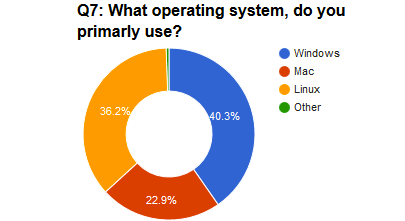
\includegraphics[width=\textwidth]{graphs/q7.png}
					\caption{Representation of results of question 7}
					\label{fig:q7}
				\end{subfigure}
				~
				\begin{subfigure}[b]{0.45\textwidth}
					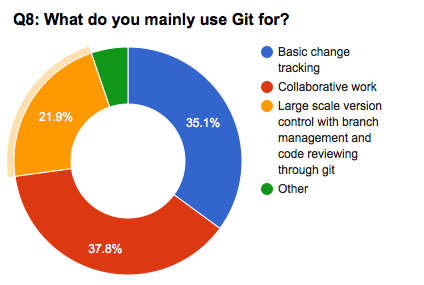
\includegraphics[width=\textwidth]{graphs/q8.png}
					\caption{Representation of results of question 8}
					\label{fig:q8}
				\end{subfigure}
				\caption{Questions 7 and 8}\label{fig:q7-q8}
			\end{figure}
			\begin{figure}[H]
				\centering
				\begin{subfigure}[b]{0.45\textwidth}
					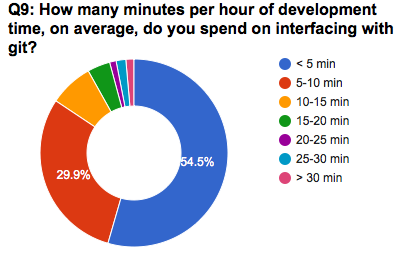
\includegraphics[width=\textwidth]{graphs/q9.png}
					\caption{Representation of results of question 9}
					\label{fig:q9}
				\end{subfigure}
				~
				\begin{subfigure}[b]{0.45\textwidth}
					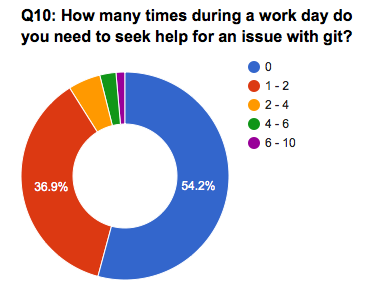
\includegraphics[width=\textwidth]{graphs/q10.png}
					\caption{Representation of results of question 10}
					\label{fig:q10}
				\end{subfigure}
				\caption{Questions 9 and 10}\label{fig:q9-q10}
			\end{figure}
			\begin{figure}[H]
				\centering
				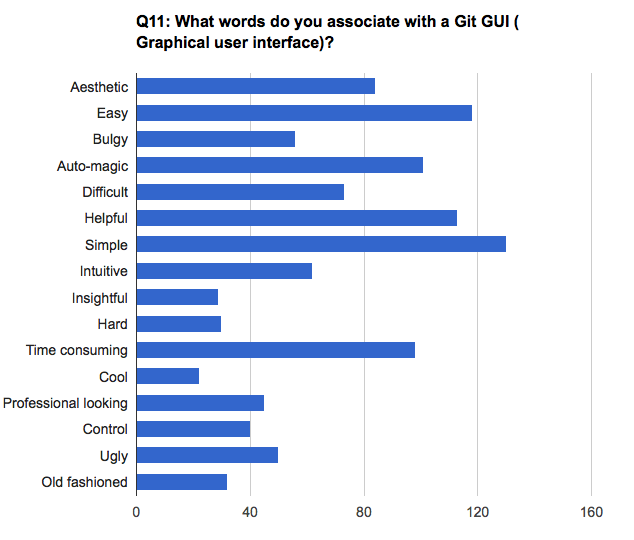
\includegraphics[width=0.8\linewidth]{graphs/q11.png}
				\caption{Representation of results of question 11}
				\label{fig:q11}
			\end{figure}
			\begin{figure}[H]
				\centering
				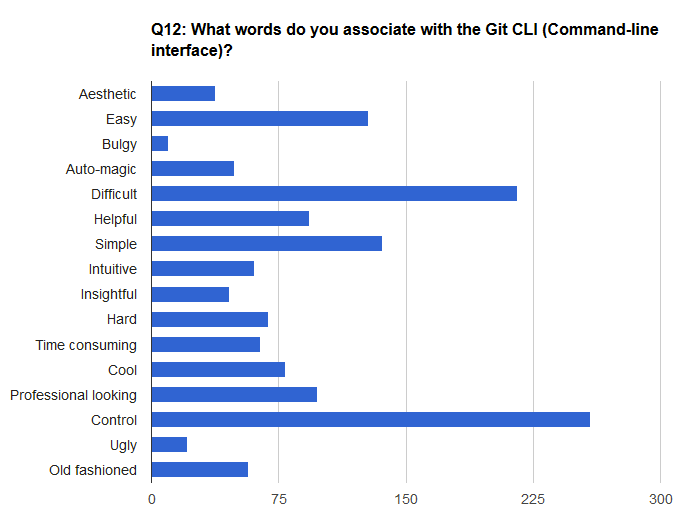
\includegraphics[width=0.8\linewidth]{graphs/q12.png}
				\caption{Representation of results of question 12}
				\label{fig:q12}
			\end{figure}
			\begin{figure}[H]
				\centering
				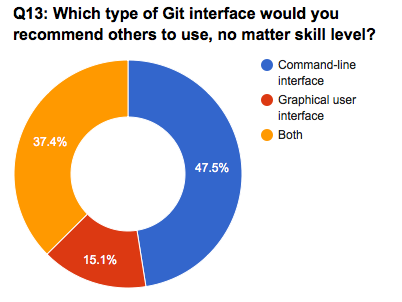
\includegraphics[width=0.5\linewidth]{graphs/q13.png}
				\caption{Representation of results of question 13}
				\label{fig:q13}
			\end{figure}
			\begin{figure}[H]
					\centering
					\begin{subfigure}[b]{0.45\textwidth}
						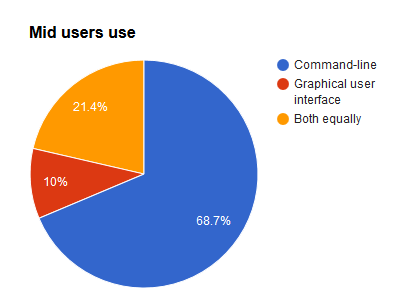
\includegraphics[width=\textwidth]{graphs/mid-users-use.png}
						\caption{Average Git users}
						\label{fig:Mid users use}
					\end{subfigure}
					~
					\begin{subfigure}[b]{0.45\textwidth}
						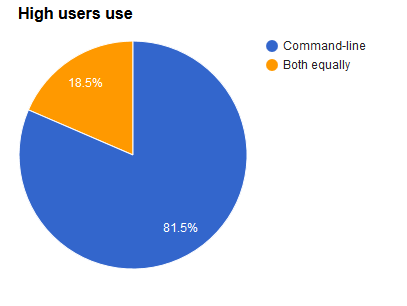
\includegraphics[width=\textwidth]{graphs/high-users-use.png}
						\caption{Very experienced Git users}
						\label{fig:High users use}
					\end{subfigure}
					\caption{The interfaces that experienced users use, according to survey result.}\label{fig:q1-q2}
				\end{figure}
				
				\begin{figure}[H]
					\centering
					\begin{subfigure}[b]{0.95\textwidth}
						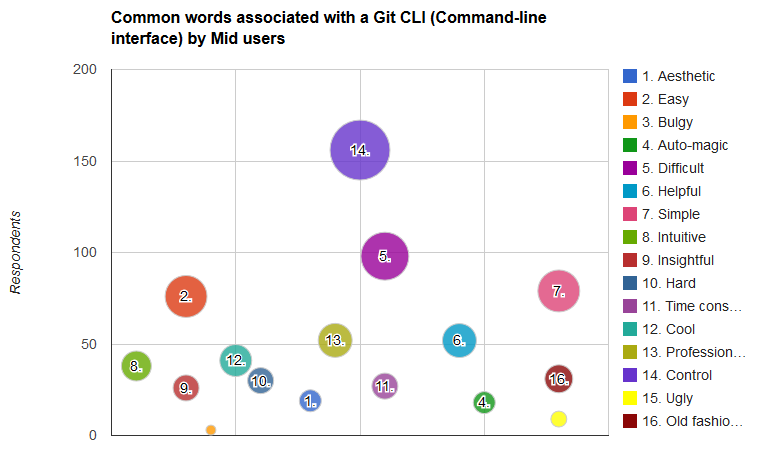
\includegraphics[width=\textwidth]{graphs/common-words-mid-users.png}
						\caption{Average Git users - common words associated with Git.}
						\label{fig:Mid users - common words associated with Git.}
					\end{subfigure}
					\caption{Common words by average Git users, in the survey, that they associate with a Git CLI.}\label{fig:q1-q2}
				\end{figure}
				
				\begin{figure}[H]
					\centering
					\begin{subfigure}[b]{0.95\textwidth}
						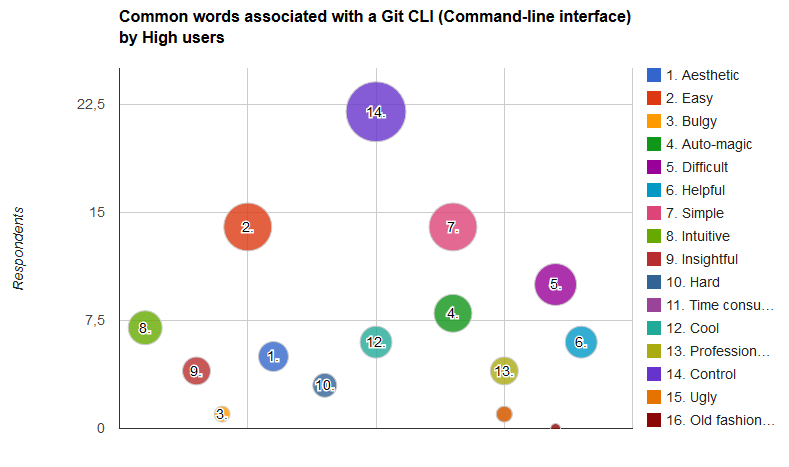
\includegraphics[width=\textwidth]{graphs/common-words-high-users.png}
						\caption{Very experienced Git users - common words associated with Git.}
						\label{fig:Mid users - common words associated with Git.}
					\end{subfigure}
					\caption{Common words by very experienced Git users, in the survey, that they associate with a Git CLI.}\label{fig:q1-q2}
				\end{figure}
			\section{Interviews}
			The interviews were conducted with three subjects, each interview lasted approximately 5-15 minutes. It was found that the demographic of low amounts of git proficiency needed a little help along to understand the questions and to elaborate on the answers. The help was given in an objective way in order to not lessen the value of the responses or skew the image in their mind, the more experienced we're a little bit more talkative and had more to say on the subject since they have had the time to test other solutions and options. 
			The full transcripts of the interviews can be found in appendix %TODO Add the acctual denominators for the interview appendixes.
			\section{User interface analysis}
				\begin{center}
					\begin{tabular}{ | p{5cm} | c | c | c | }
					\hline
					Feature & CLI & SourceTree & Smart Git HG \\ 
					\hline
					Aliases and customizing actions & Yes & Yes & No \\
					\hline
					Readability of content & Partial & Partial & Yes \\
					\hline
					Freedom of work flow construction & Yes & Partial & Partial \\
					\hline
					Ease of setup & Yes & Yes & Yes \\
					\hline
					Overview ease & Partial & Yes & Yes \\
					\hline
					Change and branch visualization & Difficult & Partial & Yes \\
					\hline
					Comprehensive searching & Difficult & Yes & Partial \\
					\hline
					\end{tabular}
					\captionof{table}{UI analysis} \label{tab:UI-Analysis}
				\end{center}
				\subsection{CLI}
				Quite a large amount of functionality in the CLI can be quite advanced, in part giving it a lot of power and flexibility but it becomes more difficult to use. Searching through the change log and files for example can quite easily become complex but the results are very flexible and thus very useful. The same goes for most of the CLI the more specific you want to be and the more demands you have on the interaction the more difficult the process becomes. This is where aliases and custom actions come in handy. They are a way for the user to write the very difficult and complex command once and then call it by an alias of their choosing. 
				\subsection{Source Tree}
				\subsection{Smart Git Hg}
		
		% Analysis
		\chapter{Analysis}
			\section{Answering the research questions}
				\subsection{RQ1: What is most commonly used when getting started with git, CLI or GUI?}
				As shown in the results chapter, in figure 5.4a the most common interface to get started in among the responders to the survey is the CLI.
				With a majority of 77,7\% percent of the respondents starting out with Git using the CLI.
				The graphical user interface is not as popular with 22,3\% of the responders stating that they got started with the GUI. 
				This result may be a linked to the common notion that in order to learn how git works it is better to start out with the CLI.
				
				
		
				\subsection{RQ2: What is most commonly used by experienced git users, CLI or GUI?}
				As demonstrated by the diagrams in figures 5.10a and 5.10b, the command-line dominates amongst the mid to highly experienced users as well. The more experienced the less often they seem to solely use a graphical user interface. This can be linked to the feeling of control felt by the users with higher experience as indicated by the diagrams in figure 5.11 and 5.12.
				In comparison to 2012's edition of the GitSurvey, 4498 respondents to the question "What Git implementation do you use?" 95\% answered "git (core) commandline" \cite{GitStructure}.
				The results makes the command-line interface appear to be the most used interface for Git amongst experienced git users.
				
		
				\subsection{RQ3 and RQ4}
		
				\subsection{RQ5: At what stage of git proficiency would you stand to gain the most from the CLI or the GUI?}
		
		% Conclusion
		\chapter{Conclusion}
		
		
		% Acknowledgment section
		\chapter*{Acknowledgement}
		
		% References section
		\newpage
		\begin{thebibliography}{1}
			
			\bibitem{GitUserSurvey}
			GitSurvey2012 - Git SCM Wiki. (2012). GitSurvey2012 - Git SCM Wiki. Available: \url{http://git.wiki.kernel.org/index.php/GitSurvey2012}. Last accessed 4th April 2015..
			
			\bibitem{MouseToRat}
			Morgan, K., Morris, R. \& Gibbs, S. (1991). When does a Mouse become a Rat? or … Comparing Performance and Preferences in Direct Manipulation and Command Line Environment. The Computer Journal. 34 (3), p265-271.
			
			\bibitem{MacVsWindows}
			Kirkpatrick, D., Sherman, S., \& Deutschman, A. (1993). Mac vs Windows. Fortune Internc\#ional. 128 (8), p57-64.
			
			\bibitem{GitInClassroom}
			Kelleher, J. (2014, 17-19 Jan). Employing git in the classroom. Paper presented at 2014 World Congress on Computer Applications and Information Systems (WCCAIS). Retrieved 4th April, 2015, at IEEE Xplore. DOI: 10.1109/WCCAIS.2014.6916568.
			
			\bibitem{Treweek}
			Treweek, P. (1996). Comparing Interfaces: Should We Assume that Ease of Use Influences Users' Preference?. Presented at Sixth Australian Conference on Computer-Human Interaction. Retrieved 4th April, 2015, at IEEE Xplore. DOI: 10.1109/OZCHI.1996.560004.
			
			% This is not being used as far as i know.
			%\bibitem{Hart}
			%Hart, D. (2009). A survey of source code management tools for programming courses. Journal of Computing Sciences in Colleges. 24 (6), p113-114.
			
			\bibitem{WrongWithGit}
			Perez De Rosso, S. \& Jackson, D. (2013). What's wrong with git?: a conceptual design analysis. Presented at 2013 ACM international symposium on New ideas, new paradigms, and reflections on programming \& software. Retrieved 4th April, 2015, at ACM Digital Library. DOI: 10.1145/2509578.2509584.
			
			\bibitem{ArtOfUnixProgramming}
			Eric S. Raymond. (2005). The Art of Unix Programming.
			Available: \url{http://www.catb.org/esr/writings/taoup/html/ch11s04.html}.
			Last accessed 6th April 2015.
			
			\bibitem{LinuxGuiVsCli}
			Juergen Haas. Linux: GUI vs. Command line. Available: \url{http://linux.about.com/cs/softofficeutility/a/gui\_cli.htm}. Last accessed 6th April 2015.
			
			\bibitem{GithubAbout}
			Github.com - Features. (2015). Available: \url{https://github.com/features/}. Last accessed 16th April 2015.
			
			\bibitem{ProGit}
			S. Chacon, Pro Git, New York, NY: Apress, 2009.
			
			\bibitem{EclipseDeveoperReport}
			The Eclipse Foundation. "Eclipse Open Source Developer Report". The Eclipse Foundation. San Francisco, CA. 2012.
			
			\bibitem{DeveloperProductivity}
			ZeroTurnaround. "Developer Productivity Report 2012: Java Tools, Tech, Devs \& Data". ZeroTurnaround. Boston, MA. 2012.
			
			\bibitem{MicrosoftSurveyResults}
			Microsoft Corporation, "Survey Results: Open Source Developer Preferences (June 2011)," Microsoft Corporation, 11 July 2011. [Online]. Available: \url{http://blogs.msdn.com/b/codeplex/archive/2011/07/11/survey-results-open-source-developer-preferences-june-2011.aspx}. [Accessed 18th April 2015].
			
			\bibitem{WhatIsGui}
			Webopedia.com. (2015). Available: \url{http://www.webopedia.com/TERM/G/Graphical\_User\_Interface\_GUI.html}. [Accessed 18th April 2015].
			
			\bibitem{FoundationVCforWebDevs}
			C. Kemper and I. Oxley. Foundation Version Control for Web Developers. Berkeley, CA: Apress. 2012.
			
			\bibitem{HistoryOfGUIWiki}
			Wikipedia. (Unknown). History of the graphical user interface. Available: \url{http://en.wikipedia.org/wiki/History_of_the_graphical_user_interface#Apple_Lisa_and_Macintosh_.28and_later.2C_the_Apple_IIgs.29}.  [Accessed 20th April 2015].
			
			\bibitem{lootcrate}
			Loot Crate. Available: \url{www.lootcrate.com} [Accessed 20th April 2015]
			
			\bibitem{GoogleSpreadsheet}
			Google Spreadsheet. Available: \url{https://www.google.se/intx/sv/work/apps/business/products/sheets/?utm_source=google&utm_medium=cpc&utm_campaign=emea-se-sv-drive-bkws-all-trial-e&utm_term=google%2Bkalkylark} [Accessed 26th April 2015]
			
			\bibitem{GitStructure}
			Unlearn what you have learned. (2014). Git: How it works. Available: \url{http://bartoz.no-ip.org/archives/2981}. [Accessed 14th May 2015].
			\bibitem{GitGUIs}
			Git SCM. GUI Clients. Available: \url{http://git-scm.com/downloads/guis}. [Accessed 14th May 2015].
			\bibitem{InTheBeginning}
			Neal Stephenson. (1999). In the Beginning was the Command Line. Available: \url{http://cristal.inria.fr/~weis/info/commandline.html}	[Accessed: 14th May 2015].	
			
		\end{thebibliography}
\end{document}